
\subsection{CAN Overview}
\paragraph{Controller Area Network (CAN)} is a standard for micro-controller and device communication. It uses messages, and was originally designed as a multiplexing method. The physical layer utilises twisted pairs (CAN+ and CAN-). Messages are framed with IDs which dictate priority. Logical 0 is Dominant and logical 1 is recessive. This means IDs that have larger values (1's in high bit places) are lower priority. Arbitration is done via first bit with a 1. All nodes see transmission.
\paragraph{Nodes} All nodes can send and receive, but not at the same time. The priority is determined by the frame ID. Messages are transmitted using non-return-to-zero (NRZ) format \\ All nodes require the following: 
\begin{itemize}
    \item Some controller :CPU/Microprocessor/host processor/micro controller
        \begin{itemize}
            \item Decides what messages mean and what to transmit
            \item Handles talking to other devices
        \end{itemize}
    \item CAN Controller
        \begin{itemize}
            \item Receiving: Stores bits until entire message is received, then can trigger interrupt for retrieval
            \item Transmitting: If the host, can send messages via CAN controller in a serial manner.
        \end{itemize}
    \item Transceiver (ISO 11898-2/3) Medium Access Unit (MAU)
        \begin{itemize}
            \item Receiving: converts at the CAN bus level for CAN controller use, protective layer for CAN controller. 
            \item Transmitting: converts bit stream from CAN controller to the CAN bus
        \end{itemize}
\end{itemize}



\subsection{CAN: IDs and arbitration}
\paragraph{ID Arbitration} When nodes transmit they see all messages including their own. If they transmit a 1 and see 0 they quit and lose arbitration. This is because 0 is dominant and they then know they do not have priority. Because of this, whenever there is a collision the lower ID will win. When a collision does happen.
The recessive message waits for the dominant message + 6-bit clocks then
attempts again
This means the first frame to transmit a 1 is the loser, thus highest
priority id frame is all 0s followed by 00\ldots.001
\paragraph{IDs as priorities}
Using ID for the type of data, or the sending node ignores the fact ID is
also used as message priority. This leads to poor real-time performance.
CAN bus is limited to around 30\% to ensure deadlines if you don't build
around the priority. Otherwise, you can achieve 70 to 80\% CAN bus usage and
have reliable deadlines.

\subsection{CAN: Bit timing}
\paragraph{Nominal Bit Time:} Time it takes to send bit components:\\

\paragraph{Synchronization} Synchronization is important to the CAN protocol. It prevents errors and allows for arbitration's to occur. Recolonization occurs every single recessive to dominant transmission during the frame. In order to sync the nominal bit time is segmented into quanta and then certain aspects can be altered to allow for synchronization. 
The nominal bit time is broken down in the following way. Each are assigned a number of quanta. For example a system where we break our nominal bit time into 10 quanta.


Sync (1 quanta)

Propagation (3 quanta)

Phase segment 1 (3 quanta)
 
Phase segment 2 (3 quanta)


Synchronization occurs as follows. 

\begin{enumerate}
\def\labelenumi{\arabic{enumi}.}
\item
  \textbf{Bus Idle} -\textgreater{} wait for first recessive to dominant
  transition
\item
 \textbf{ Hard synchronization}
\item
  \textbf{Resync} occurs on every recessive to dominant transition during the
  frame (message?)

  \begin{enumerate}
  \def\labelenumii{\alph{enumii}.}
  \item
    CAN controller expects this at multiple of nominal bit time.
  \item
    Else It adjust nominal bit time accordingly.
  \end{enumerate}
\end{enumerate}

~

\paragraph{Resync and Adjustment process:}

\begin{itemize}
\item
  Produce a number of quanta to divide the bits\textquotesingle{}
  segments into time slices.

  \begin{itemize}
  \item
    The number of quanta can vary based on the controller
  \item
    The quantity of quanta a segment is assigned can vary depending on
    system needs
  \end{itemize}
\item
  On out-of-sync (before or after) transition controller calculates the time
  difference, to compensate:

  \begin{itemize}
  \item
    If we need to lengthen we do so to phase 1
  \item
    If we need to reduce time we do so in phase 2.
  \end{itemize}
\item
  As a result of either a or b, we have adjusted the timing of the
  receiver to the transmitting node and synchronized them.
\item
  We continuously do so at every recessive to dominant transition to
  keep synchronization

  \begin{itemize}
  \item
    This reduces errors induced by noise (random error)
  \item
    Allows for resync to nodes that lost arbitration back to the one
    that won previously.
  \item
  \end{itemize}
\end{itemize}

\subsection{CAN Protocol Layers:}
\begin{itemize}
    \item Application layer
    \item Object layer
    \item Transfer layer
    \item Physical layer
\end{itemize}


We are building the transfer layer?

~

\subsubsection{CAN Transfer layer:}

\begin{itemize}
\item
  Most of the CAN standard applies to this layer, it is what receives
  messages from the physical layer and into the object layer for use in
  the application.
\item
  Transfer layer is responsible for:

  \begin{itemize}
  \item
    Synchronization
  \item
    Bit timing
  \item
    Message framing
  \item
    Arbitration
  \item
    Acknowledgement
  \item
    Error Detection
  \item
    Signalling
  \item
    Confinement
  \end{itemize}
\item
  To accomplish the previous responsibilities, it performs the following
  tasks:

  \begin{itemize}
  \item
    Fault confinement
  \item
    Error detection
  \item
    Message Validation
  \item
    Arbitration
  \item
    Message framing
  \item
    Transfer rate and timing
  \item
    Information routing
  \end{itemize}
\end{itemize}

~

Physical layer

\begin{itemize}
\item
  Pinout:

  \begin{itemize}
  \item
    Pin 2: CAN- (Low)
  \item
    Pin 3: GND
  \item
    Pin 7: CAN+ (High)
  \item
    Pin 9: CAN V+ (power)
  \end{itemize}
\end{itemize}

\begin{quote}
~
\end{quote}

\subsection{CAN Frames:}

\begin{itemize}
\item
  Two types of frame format

  \begin{enumerate}
  \def\labelenumi{\arabic{enumi}.}
  \item
    Base frame format

    \begin{enumerate}
    \def\labelenumii{\roman{enumii}.}
    \item
      11- bits for identifier
    \item
      IDE bit dominant
    \end{enumerate}
  \item
    Extended frame format

    \begin{enumerate}
    \def\labelenumii{\roman{enumii}.}
    \item
      11- bit identifier + 18-bit extension = 29-bit identifier
    \item
      IDE bit recessive
    \end{enumerate}
  \end{enumerate}
\item
  There are four types of frames.
\item
  Regardless of type all begin with a start of frame (SOF) bit to signal
  start of frame transmission.
\item
  Frame types:

  \begin{enumerate}
  \def\labelenumi{\arabic{enumi}.}
  \item
    Data Frame: a frame containing node data for transmission
    .

  \item
    Remote frame: requests transmission of an identifier
  \item
    Error frame: frame type for any node detecting an error.
  \item
    Overload frame: a buffer/delay for data or remote frame.
  \end{enumerate}
\end{itemize}
\begin{figure}
    \centering
    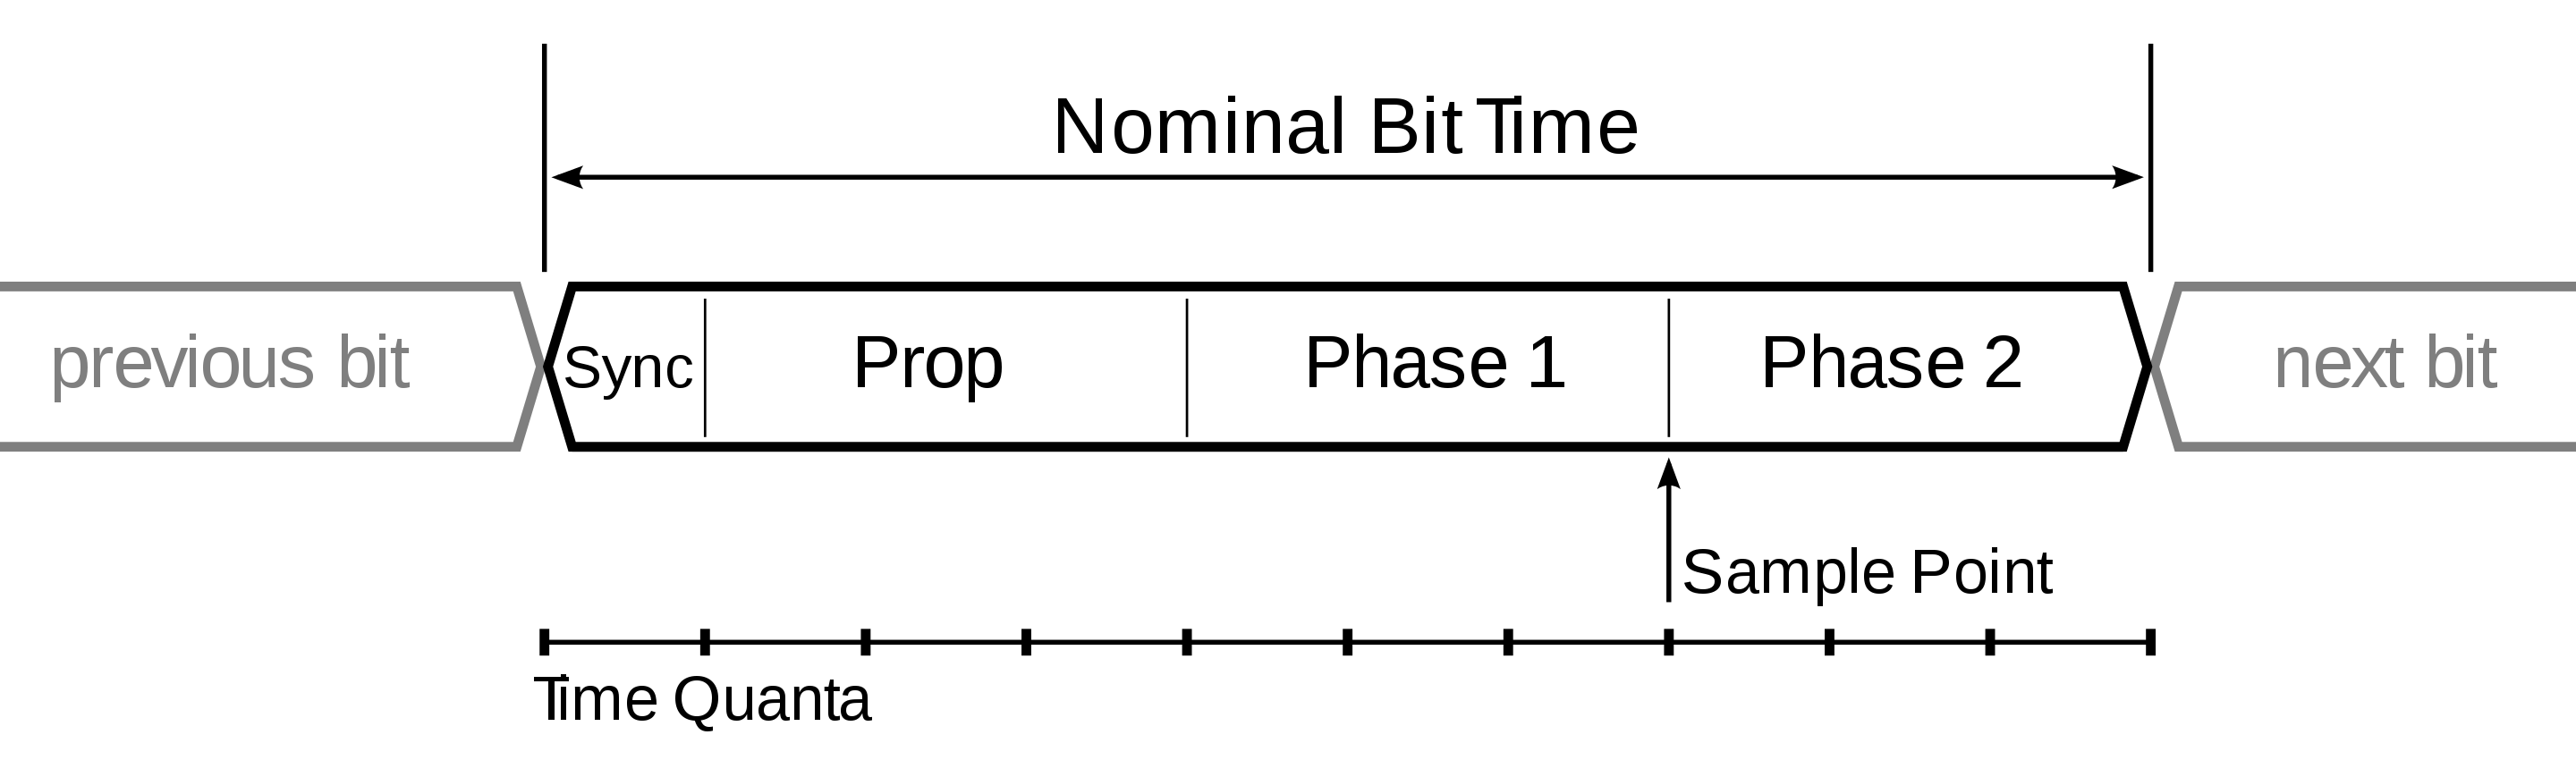
\includegraphics[width=1\linewidth]{2880px-CAN_Bit_Timing2.svg.png}
    \caption{CAN Bit Timing: Wikipedia}
    \label{fig:enter-label}
\end{figure}
\begin{figure}
      \centering
      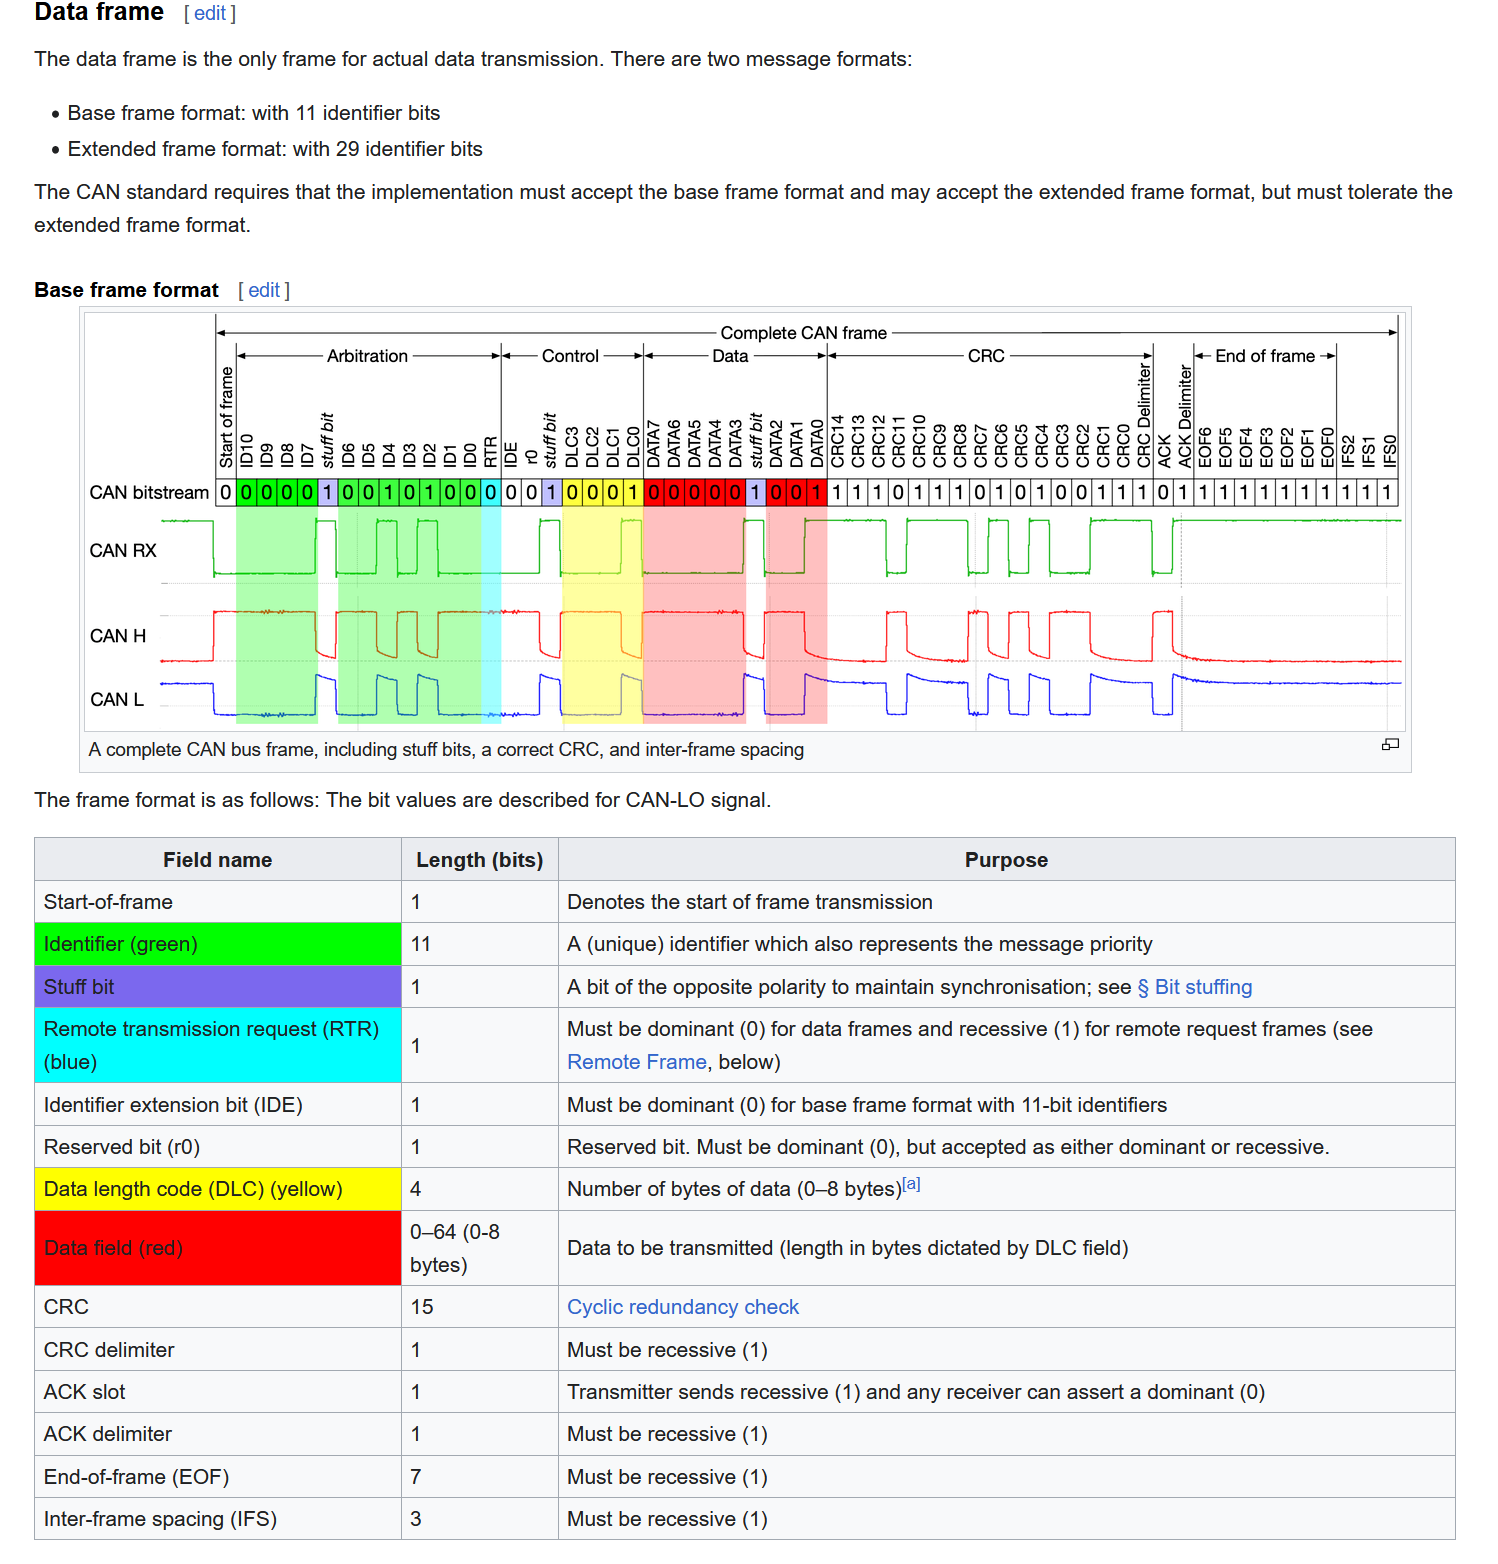
\includegraphics[width=1\linewidth]{Dataframe.png}
      \caption{Data frame: Wikipedia}
      \label{fig:enter-label}
  \end{figure}



